
\section{Choropleth Maps}
\label{sec-1}
\label{sec:multiChoropleth}
A choropleth map shades regions according to the measurement of a
variable displayed on the map. The choropleth map is an appropiate
tool to visualize a variable uniformly distributed within each
region, changing only at the region boundaries. This method
performs correctly with homogeneous regions, both in size and
shape.  

This section details how to create a multivariate choropleth map to
show the results of the 2011 Spanish general elections. It is inspired
by the infographic from the \emph{New York Times\footnote{\url{http://www.nytimes.com/interactive/2009/03/10/us/20090310-immigration-explorer.html}}}, a multivariate
choropleth map of the inmigration behavior in the United States.

\lstset{language=R,numbers=none}
\begin{lstlisting}
votes2011 <- read.csv('data/votes2011.csv',
		      colClasses=c('factor', 'factor', 'numeric', 'numeric'))
\end{lstlisting}

The next section describes how to define a \texttt{SpatialPolygonsDataFrame}
with the data from this \texttt{data.frame} and the spatial information of
the administrative boundaries from a shapefile. You can skip it for
later reading if you are not interested in this procedure and jump to
the section \ref{sec:map} where the maps are produced.

\subsection{\floweroneleft Administrative Boundaries}
\label{sec-1-1}

The Spanish administrative boundaries are available as shapefiles at
the INE (Instituto Nacional de Estadística) webpage\footnote{\url{http://www.ine.es/} > Products and services > Publications > Download the PC-Axis program > Municipal maps}. Both the
municipalities, \texttt{espMap}, and province boundaries, \texttt{provinces}, are
read as \texttt{SpatialPolygonsDataFrame} with \texttt{readShapePoly}.

\index{Packages!maps@\texttt{maps}}
\index{Packages!maptools@\texttt{maptools}}
\index{Packages!rgeos@\texttt{rgeos}}
\index{Packages!sp@\texttt{sp}}
\index{Packages!latticeExtra@\texttt{latticeExtra}}

\lstset{language=R,numbers=none}
\begin{lstlisting}
library(sp)
library(maptools)
\end{lstlisting}

\index{INE}
\index{readShapePoly@\texttt{readShapePoly}}
\index{Encoding@\texttt{Encoding}}

\lstset{language=R,numbers=none}
\begin{lstlisting}
old <- setwd(tempdir())
download.file('http://goo.gl/TIvr4', 'mapas_completo_municipal.rar')
system2('unrar', c('e', 'mapas_completo_municipal.rar'))
espMap <- readShapePoly(fn="esp_muni_0109")
Encoding(levels(espMap$NOMBRE)) <- "latin1"

provinces <- readShapePoly(fn="spain_provinces_ag_2")
setwd(old)
\end{lstlisting}

Some of the polygons are repeated and can be dissolved with
\texttt{unionSpatialPolygons} (the \texttt{rgeos} package must be installed).
\index{unionSpatialPolygons@\texttt{unionSpatialPolygons}}
\lstset{language=R,numbers=none}
\begin{lstlisting}
## dissolve repeated polygons
espPols <- unionSpatialPolygons(espMap, espMap$PROVMUN)
\end{lstlisting}

Spanish maps are commonly displayed with the Canarian islands next
to the peninsula. First we have to extract the polygons of the
islands and the polygons of the peninsula, and then shift the
coordinates of the islands with \texttt{elide}. Finally, a new
\texttt{SpatialPolygons} object binds the shifted islands with the
peninsula.

\lstset{language=R,numbers=none}
\begin{lstlisting}
## Extract Canarias islands from the SpatialPolygons object
canarias <-  sapply(espPols@polygons, function(x)substr(x@ID, 1, 2) %in% c("35",  "38"))
peninsulaPols <- espPols[!canarias]
islandPols <- espPols[canarias]

## Shift the island extent box to position them at the bottom right corner
dy <- bbox(peninsulaPols)[2,1] - bbox(islandPols)[2,1]
dx <- bbox(peninsulaPols)[1,2] - bbox(islandPols)[1,2]
islandPols2 <- elide(islandPols, shift=c(dx, dy))
bbIslands <- bbox(islandPols2)

## Bind Peninsula (without islands) with shifted islands
espPols <- rbind(peninsulaPols, islandPols2)
\end{lstlisting}

The final step is to link the data with the polygons. The \texttt{ID} slot of
each polygon is the key to find the correspondent registry in the
\texttt{votes2011} dataset.
\lstset{language=R,numbers=none}
\begin{lstlisting}
## Match polygons and data using ID slot and PROVMUN column
IDs <- sapply(espPols@polygons, function(x)x@ID)
idx <- match(IDs, votes2011$PROVMUN)

##Places without information
idxNA <- which(is.na(idx))

##Information to be added to the SpatialPolygons object
dat2add <- votes2011[idx, ]

## SpatialPolygonsDataFrame uses row names to match polygons with data
row.names(dat2add) <- IDs
espMapVotes <- SpatialPolygonsDataFrame(espPols, dat2add)

## Drop those places without information
espMapVotes <- espMapVotes[-idxNA, ]
\end{lstlisting}
\subsection{Map}
\label{sec-1-2}
\label{sec:map}
The \texttt{SpatialPolygonsDataFrame} constructed in the previous section
contains two main variables: \texttt{whichMax}, the name of the predominant
political option, and \texttt{pcMax}, the percentage of votes obtained by
this political option.

\texttt{whichMax} is a categorical value with four levels: the two main
parties (\texttt{PP} and \texttt{PSOE}), the abstention results (\texttt{ABS}), and the
rest of the parties (\texttt{OTH}). Figure \ref{fig:whichMax} encodes these levels
with a qualitative palette with constant hues and varying chroma and
luminance for each class using the package \texttt{colorspace}
\cite{Zeileis.Hornik.ea2009}. In order to improve the color
discrimination, hues are equally spaced along the HCL (Hue, Chroma,
Luminance) based color wheel.

\index{Packages!colorspace@\texttt{colorspace}}
\index{rainbow_hcl@\texttt{rainbow\_hcl}}
\lstset{language=R,numbers=none}
\begin{lstlisting}
library(colorspace)  

classes <- levels(factor(espMapVotes$whichMax))
nClasses <- length(classes)

qualPal <- rainbow_hcl(nClasses, start=30, end=300)
\end{lstlisting}

For the definition of a combined palette in the next section, it is
interesting to note that the colors provided by \texttt{rainbow\_hcl} can be
obtained with the following code where the distances between hues and
their values are computed explicitly.
\index{hcl@\texttt{hcl}}
\lstset{language=R,numbers=none}
\begin{lstlisting}
## distance between hues
step <- 360/nClasses 
## hues equally spaced
hue = (30 + step*(seq_len(nClasses)-1))%%360 
qualPal <- hcl(hue, c=50, l=70)
\end{lstlisting}

\lstset{language=R,numbers=none}
\begin{lstlisting}
spplot(espMapVotes["whichMax"], col='transparent', col.regions=qualPal)
\end{lstlisting}

\begin{figure}[htb]
\centering
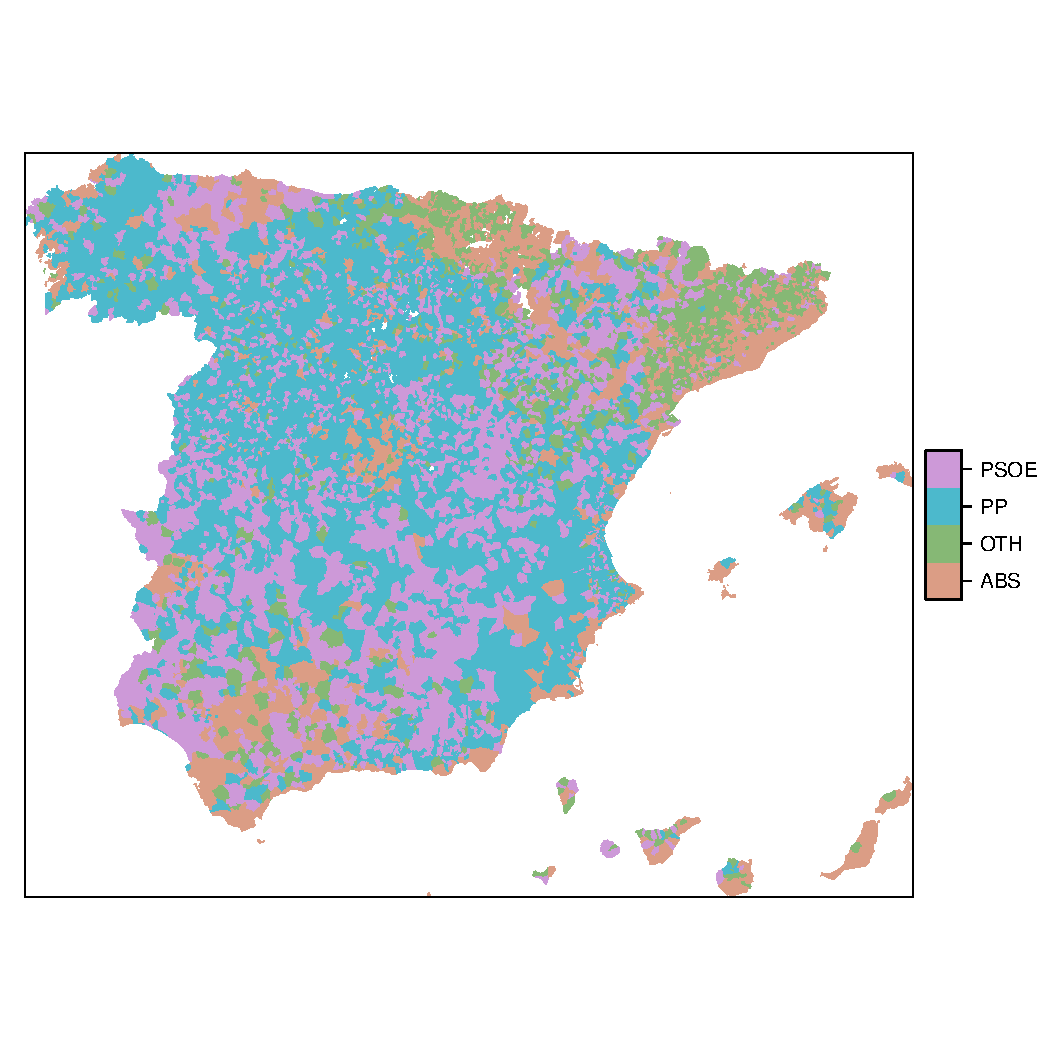
\includegraphics[width=.9\linewidth]{figs/whichMax.pdf}
\caption{\label{fig:whichMax}Categorical choropleth map displaying the name of the predominant political option in each municipality in the 2011 Spanish general elections.}
\end{figure}

On the other hand, \texttt{pcMax} is a quantitative variable that can be
adequately displayed with a sequential palette (Figure \ref{fig:pcMax}).
\lstset{language=R,numbers=none}
\begin{lstlisting}
quantPal <- rev(heat_hcl(16))
spplot(espMapVotes["pcMax"], col='transparent', col.regions=quantPal)
\end{lstlisting}

\begin{figure}[htb]
\centering
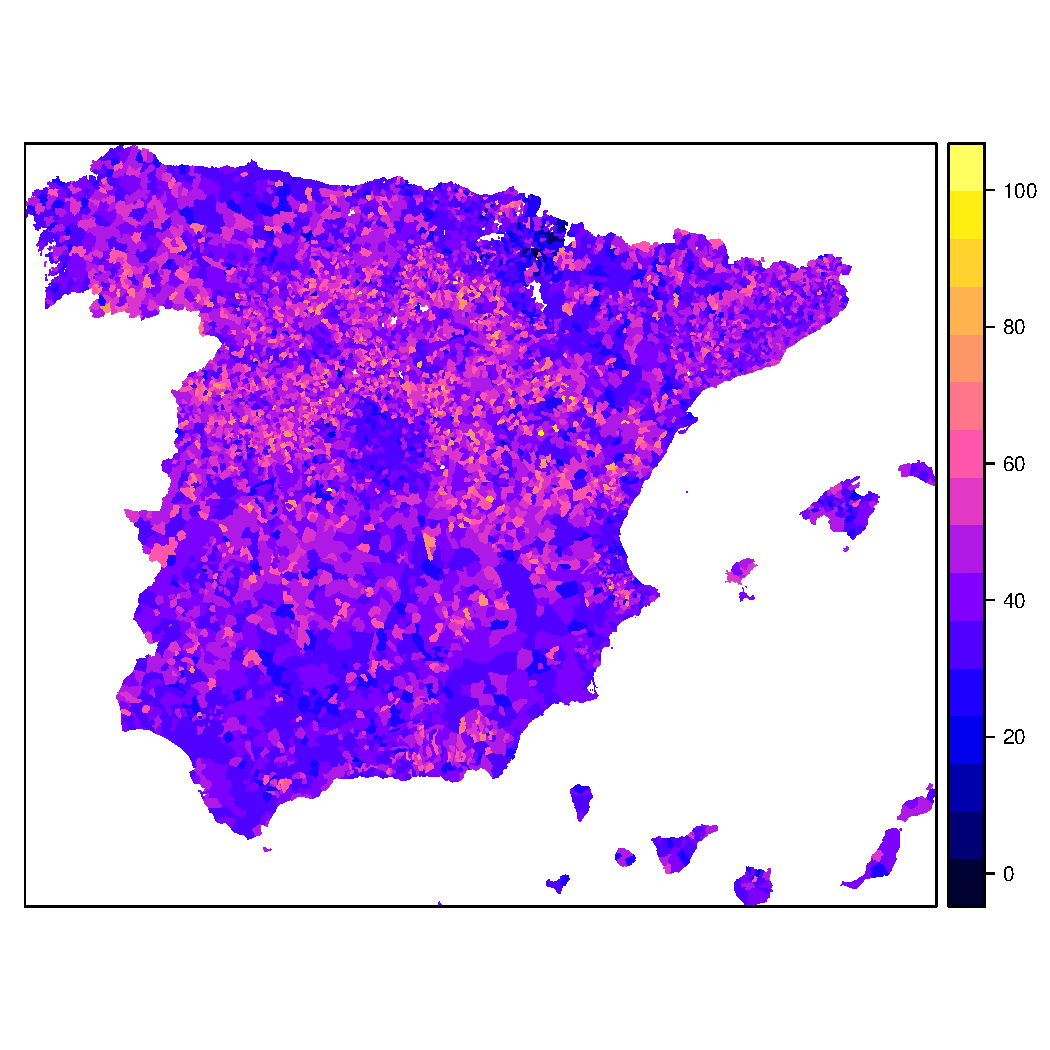
\includegraphics[width=.9\linewidth]{figs/pcMax.pdf}
\caption{\label{fig:pcMax}Quantitative choropleth map displaying the percentage of votes obtained by the predominant political option in each municipality in the 2011 Spanish general elections.}
\end{figure}
\subsection{\floweroneleft Categorical and Quantitative Variables Combined in a Multivariate Choropleth Map}
\label{sec-1-3}
Following the inspiring example of the infographic from the \emph{New
York Times}, we will combine both choropleth maps to produce a
multivariate map: the hue of each polygon will be determined by
the name of the predominant option (\texttt{whichMax}) but the chroma and
luminance will vary according to the percentage of votes
(\texttt{pcMax}). Hues are computed with the same method as in Figure
\ref{fig:whichMax}, while the corresponding values of chroma and
luminance are calculated with the \texttt{sequential\_hcl} function.

\index{sequential_hcl@\texttt{sequential\_hcl}}
\lstset{language=R,numbers=none}
\begin{lstlisting}
classes <- levels(factor(espMapVotes$whichMax))
nClasses <- length(classes)
step <- 360/nClasses
multiPal <- lapply(1:nClasses, function(i){
    rev(sequential_hcl(16, h = (30 + step*(i-1))%%360))
    })
\end{lstlisting}

With this multivariate palette we can produce a list of maps
extracting the polygons according to each class and filling with
the appropiate color from this palette. The resulting list of
\texttt{trellis} objects can be combined with \texttt{Reduce} and the
\texttt{+.trellis} function of the \texttt{latticeExtra} and produce a \texttt{trellis}
object.

It is important to note that, to ensure the legend's homogeneity, the
breakpoints defined by the \texttt{at} argument are the same for all the
individual maps.

\index{Reduce@\texttt{Reduce}} \index{spplot@\texttt{spplot}}
\lstset{language=R,numbers=none}
\begin{lstlisting}
pList <- lapply(1:nClasses, function(i){
    ## Only those polygons corresponding to a level are selected
    mapClass <- espMapVotes[espMapVotes$whichMax==classes[i],]
    pClass <- spplot(mapClass['pcMax'], col.regions=multiPal[[i]],
		     col='transparent',
		     ## labels only needed in the last legend
		     colorkey=(if (i==nClasses) TRUE else list(labels=rep('', 6))),
		     at = seq(0, 100, by=20))
})

p <- Reduce('+', pList)
\end{lstlisting}

The legend of this \texttt{trellis} object must be defined
manually. The main operation is to merge the legends from the
components of the list of maps to obtain a bivariate
legend. 

The first step is to add a title to each individual legend.  This is a
little complex because \texttt{levelplot} (the engine under the \texttt{spplot}
method) does not include a title in its color key. The solution is to
define a function to add the title and include it as an argument to
the legend component of each \texttt{trellis} object. The \texttt{print.trellis}
method will process this function when displaying the \texttt{trellis}
object. The \texttt{frameGrob} and \texttt{packGrob} of the \texttt{grid} package will do
the main work inside this function.

\index{textGrob@\texttt{textGrob}}
\index{packGrob@\texttt{packGrob}}
\index{Packages!grid@\texttt{grid}}
\lstset{language=R,numbers=none}
\begin{lstlisting}
## Function to add a title to a legend
addTitle <- function(legend, title){
  titleGrob <- textGrob(title, gp=gpar(fontsize=8), hjust=1, vjust=1)
  ## retrieve the legend from the trellis object
  legendGrob <- eval(as.call(c(as.symbol(legend$fun), legend$args)))
  ## Layout of the legend WITH the title
  ly <- grid.layout(ncol=1, nrow=2,
		    widths=unit(0.9, 'grobwidth', data=legendGrob))
  ## Create a frame to host the original legend and the title
  fg <- frameGrob(ly, name=paste('legendTitle', title, sep='_'))
  ## Add the grobs to the frame
  pg <- packGrob(fg, titleGrob, row=2)
  pg <- packGrob(pg, legendGrob, row=1)
  }

## Access each trellis object from pList...
for (i in seq_along(classes)){
  ## extract the legend (automatically created by spplot)...
  lg <- pList[[i]]$legend$right
  ## ... and add the addTitle function to the legend component of each trellis object
  pList[[i]]$legend$right <- list(fun='addTitle',
				  args=list(legend=lg, title=classes[i]))
}
\end{lstlisting}

Now that every component of \texttt{pList} includes a legend with a title,
the legend of the \texttt{p} trellis object can be modified to store the
merged legends from the set of components of \texttt{pList}.

\lstset{language=R,numbers=none}
\begin{lstlisting}
## List of legends
legendList <- lapply(pList, function(x){
  lg <- x$legend$right
  clKey <- eval(as.call(c(as.symbol(lg$fun), lg$args)))
  clKey
})

## Function to pack the list of legends in a unique legend
## Adapted from latticeExtra::: mergedTrellisLegendGrob
packLegend <- function(legendList){
  N <- length(legendList)
  ly <- grid.layout(nrow = 1,  ncol = N)
  g <- frameGrob(layout = ly, name = "mergedLegend")
  for (i in 1:N) g <- packGrob(g, legendList[[i]], col = i)
  g
}

## The legend of p will include all the legends
p$legend$right <- list(fun = 'packLegend',  args = list(legendList = legendList))
\end{lstlisting}

Figure \ref{fig:mapLegends} displays the result with the province boundaries
superposed (only for the peninsula due to a problem with the
definition of boundaries the Canarian islands in the file) and a
rectangle to separate the Canarian islands from the remainder of the
map.

\lstset{language=R,numbers=none}
\begin{lstlisting}
canarias <- provinces$PROV %in% c(35, 38)
peninsulaLines <- provinces[!canarias,]

p +
  layer(sp.polygons(peninsulaLines,  lwd = 0.1)) +
  layer(grid.rect(x=bbIslands[1,1], y=bbIslands[2,1],
		  width=diff(bbIslands[1,]),
		  height=diff(bbIslands[2,]),
		  default.units='native', just=c('left', 'bottom'),
		  gp=gpar(lwd=0.5, fill='transparent')))
\end{lstlisting}

\begin{figure}[htb]
\centering
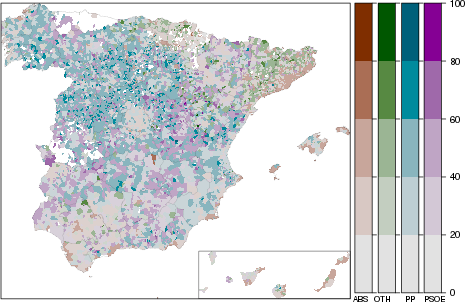
\includegraphics[width=.9\linewidth]{figs/mapLegends.png}
\caption{\label{fig:mapLegends}Spanish general elections results. The map shows the result of the most voted option in each municipality.}
\end{figure}
